\part{Fundamental electromagnetic principles}
\title[Fundamental electromagnetic principles]{Fundamental electromagnetic principles}  
\date{}  
\frame{\titlepage} 

%%%%%%%%%%%%%%%%%%%%%%%%%%%%%%%%%%%%%%%%%%%%%%%%%%%%%%%%%%%%%
%% Ampere's circuital law: magnetic field strength %%
%%%%%%%%%%%%%%%%%%%%%%%%%%%%%%%%%%%%%%%%%%%%%%%%%%%%%%%%%%%%%
\begin{frame}
	\frametitle{Amp\`ere's circuital law: magnetic field strength}
	\begin{columns}
		\begin{column}{0.55\textwidth}
			Relates the circulation of a magnetic field around a closed loop to the electric current passing through the loop:
            \begin{align}
                \mbox{Integral form:} \quad &\oint_{\mathcal{C}} \bm{H} \cdot \mathrm{d}\bm{l} = I_{\mathrm{f}},\\
                \mbox{Differential form:} \quad &\nabla \times \bm{H} = \bm{J}_{\mathrm{f}}. 
            \end{align}
            Here, $\bm{H}$ is the magnetic field strength, $\bm{J}_{\mathrm{f}}$ is the free current density, and $I_{\mathrm{f}}$ is the free current enclosed by the loop $\mathcal{C}$. 
            \vspace{0.25cm}
            \begin{itemize}
                \item Free current: current that is not bound to a material (i.e., without polarization and magnetization currents).
                \item SI-unit: $[H] = \si{\ampere}$
            \end{itemize}
		\end{column}
        \hfill
		\begin{column}{0.4\textwidth}
			\begin{figure}
				\centering
				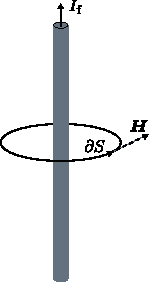
\includegraphics[height=0.7\textheight]{fig/lec02/Magnetic_field_strength_simple_conductor.pdf}
				\caption{Illustration of the magnetic field strength $\bm{H}$ around a simple conductor}
			\end{figure}
		\end{column}
		\end{columns}
\end{frame}

%%%%%%%%%%%%%%%%%%%%%%%%%%%%%%%%%%%%%%%%%%%%%%%%%%%%%%%%%%%%%
%% Ampere's circuital law %%
%%%%%%%%%%%%%%%%%%%%%%%%%%%%%%%%%%%%%%%%%%%%%%%%%%%%%%%%%%%%%
\begin{frame}
	\frametitle{Amp\`ere's circuital law: magnetic field strength example}
	\begin{columns}
		\begin{column}{0.55\textwidth}
			What is the free current $I_{\mathrm{f}}$ enclosed by the loop $\mathcal{C}$?
            \begin{itemize}
                \item The current $I_1$ flows in the direction of the loop $\mathcal{C}$ (according to right-hand rule).
                \item The current $I_1$ must be counted $N$ times due to the $N$ turns of wire around the loop $\mathcal{C}$.
                \item The current $I_2$ flows in the opposite direction of the loop $\mathcal{C}$ (according to right-hand rule).
                \item Result:
            \end{itemize}
            \vspace{0.25cm}
            \begin{equation*}
                I_\mathrm{f} = N \cdot I_1 - I_2.
            \end{equation*}
		\end{column}
        \hfill
		\begin{column}{0.45\textwidth}
			\begin{figure}
				\centering
				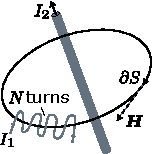
\includegraphics[height=0.5\textheight]{fig/lec02/Magnetic_field_strength_multiple_conductors.pdf}
				\caption{Arrangement with two electrical conductors}
			\end{figure}
		\end{column}
		\end{columns}
\end{frame}

%%%%%%%%%%%%%%%%%%%%%%%%%%%%%%%%%%%%%%%%%%%%%%%%%%%%%%%%%%%%%
%% Ampere's circuital law: magnetic flux %%
%%%%%%%%%%%%%%%%%%%%%%%%%%%%%%%%%%%%%%%%%%%%%%%%%%%%%%%%%%%%%
\begin{frame}
	\frametitle{Magnetic flux and flux linkage}
	\begin{columns}
		\begin{column}{0.575\textwidth}
			Variant for magnetic flux density $\bm{B}$:
            \begin{align}
                \mbox{Integral form:} \quad &\oint_{\mathcal{C}} \bm{B} \cdot \mathrm{d}\bm{l} = \mu_0 I,\\
                \mbox{Differential form:} \quad &\nabla \times \bm{B} = \mu_0\bm{J}. 
            \end{align}
            Here, $\mu_0$ is the permeability of free space, $\bm{J}$ is the total current density and $I$ is the total current enclosed by the loop $\mathcal{C}$. 
            \vspace{0.25cm}
            \begin{itemize}
                \item SI-unit: $[B] = \si{\tesla} = \si{\kilogram\per\ampere\second\squared}$
                \item Example contour $\mathcal{C}$  on the right covering $N$ turns and length $l$ (flux density within solenoid):
            \end{itemize}
            $$\oint_{\mathcal{C}} \bm{B} \cdot \mathrm{d}\bm{l} = N \mu_0 I  \Leftrightarrow B = \frac{N \mu_0 I}{l}$$
		\end{column}
        \hfill
		\begin{column}{0.425\textwidth}
            \vspace{-0.2cm}
			\begin{figure}
				\centering
				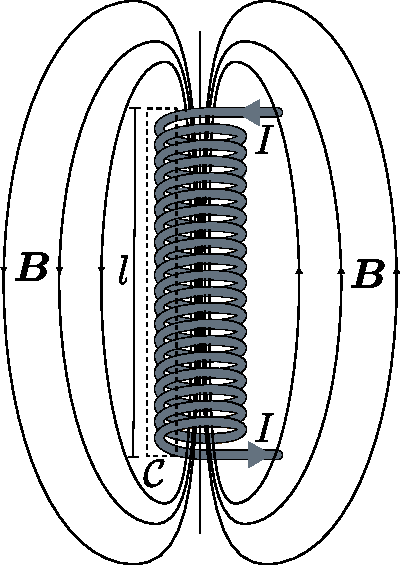
\includegraphics[height=0.68\textheight]{fig/lec02/Solenoid_Ampere_law.pdf}
				\caption{Magnetic flux $\Phi$ evaluated at the surface $\bm{S}$  (adapted from: \href{https://commons.wikimedia.org/wiki/File:Solenoid_and_Ampere_Law.png}{Wikimedia Commons}, Goodphy, \href{https://creativecommons.org/licenses/by-sa/4.0/deed.en}{CC BY-SA 4.0})}
			\end{figure}
		\end{column}
		\end{columns}
\end{frame}

%%%%%%%%%%%%%%%%%%%%%%%%%%%%%%%%%%%%%%%%%%%%%%%%%%%%%%%%%%%%%
%% Ampere's circuital law: magnetic flux %%
%%%%%%%%%%%%%%%%%%%%%%%%%%%%%%%%%%%%%%%%%%%%%%%%%%%%%%%%%%%%%
\begin{frame}
	\frametitle{Magnetic flux and flux linkage}
	\begin{columns}
		\begin{column}{0.575\textwidth}
			The magnetic flux $\Phi$ is the surface integral of the normal component of $\bm{B}$ over that surface:
            \begin{align}
                \Phi = \int_{S} \bm{B} \cdot \mathrm{d}\bm{S}. 
            \end{align}
            As there are no magnetic monopoles, the magnetic flux through a closed surface (which is covering a volume without holes) is always zero:
            \begin{align}
                \oint_{S} \bm{B} \cdot \mathrm{d}\bm{S} = 0.
            \end{align}
            The flux linkage $\Psi$ is the product of the magnetic flux $\Phi$ and the number of turns $N$ of a coil:
            \begin{align}
                \Psi = N  \Phi.
            \end{align}
		\end{column}
        \hfill
		\begin{column}{0.425\textwidth}
            \vspace{-0.2cm}
			\begin{figure}
				\centering
				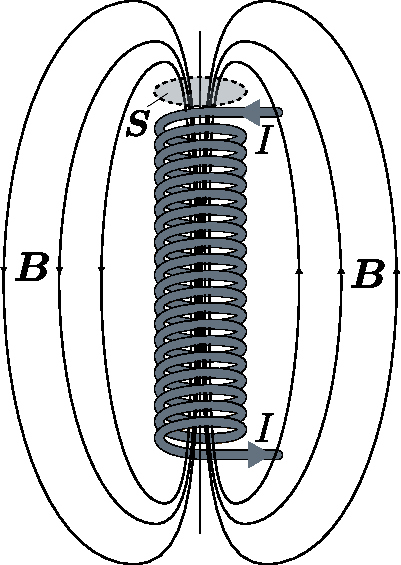
\includegraphics[height=0.68\textheight]{fig/lec02/Solenoid_Flux.pdf}
				\caption{Magnetic flux $\Phi$ evaluated at the surface $\bm{S}$  (adapted from: \href{https://commons.wikimedia.org/wiki/File:Solenoid_and_Ampere_Law.png}{Wikimedia Commons}, Goodphy, \href{https://creativecommons.org/licenses/by-sa/4.0/deed.en}{CC BY-SA 4.0})}
			\end{figure}
		\end{column}
		\end{columns}
\end{frame}

%%%%%%%%%%%%%%%%%%%%%%%%%%%%%%%%%%%%%%%%%%%%%%%%%%%%%%%%%%%%%
%% Boosting the magnet field with ferromagnetic materials %%
%%%%%%%%%%%%%%%%%%%%%%%%%%%%%%%%%%%%%%%%%%%%%%%%%%%%%%%%%%%%%
\begin{frame}
	\frametitle{Boosting the magnet field with ferromagnetic materials}
	\begin{columns}
		\begin{column}{0.575\textwidth}
			While $\bm{H}$ depends on the free currents applied to an object, $\bm{B}$ depends on the material properties of the object. In free space (vacuum), the relation is linear and represented by the magnetic constant $\mu_0$:
            \begin{align}
                \bm{B} = \mu_0 \bm{H} \quad \mbox{with} \quad \mu_0 \approx \SI{4 \pi e-7}{\newton\per\ampere\squared}.
            \end{align}
            To boost $\bm{B}$ for a given $\bm{H}$, ferromagnetic materials are typically used. These materials have a high relative magnetic permeability $\mu_{\mathrm{r}}$:
            \begin{align}
                \bm{B} = \mu \bm{H} = \mu_0 \mu_{\mathrm{r}} \bm{H}.
                \label{eq:linear_permeability} 
            \end{align}
            Note that $\mu_{\mathrm{r}}$ is a dimensionless quantity and that \eqref{eq:linear_permeability} assumes linear and isotropic material behavior.
		\end{column}
        \hfill
		\begin{column}{0.425\textwidth}
            \vspace{-0.2cm}
			\begin{figure}
				\centering
				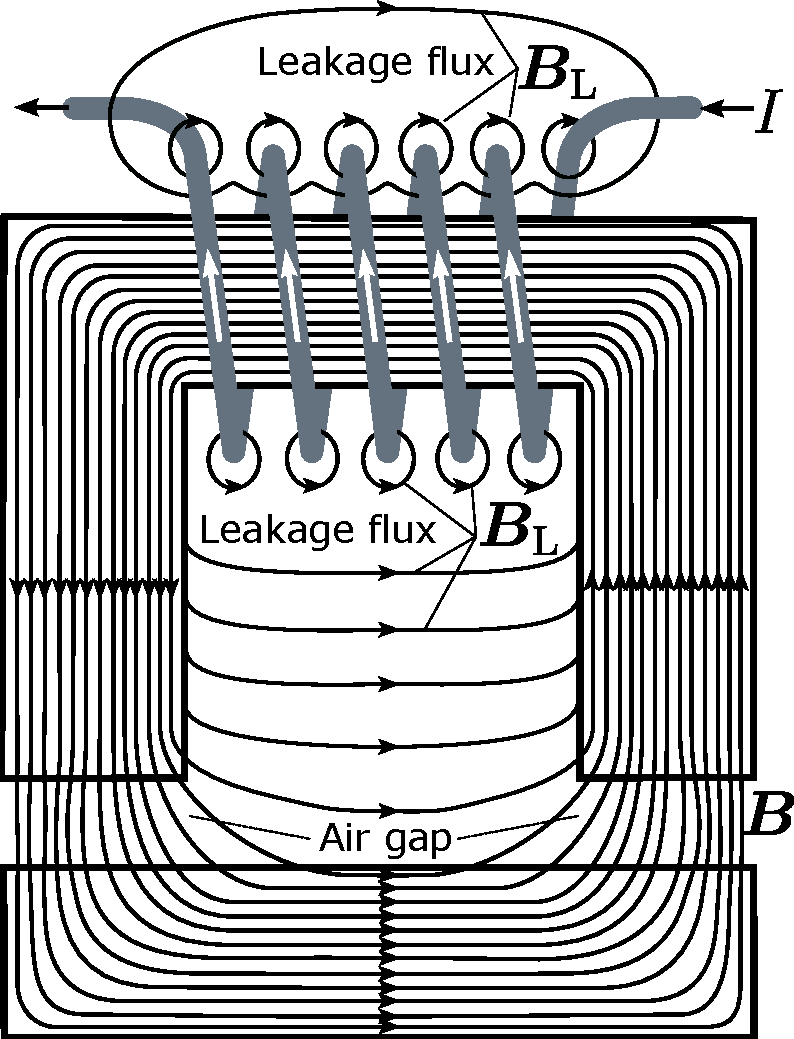
\includegraphics[height=0.68\textheight]{fig/lec02/Electromagnet_with_gap.pdf}
				\caption{Simplified magnetic field lines of an iron yoke with a coil  (adapted from: \href{https://en.m.wikipedia.org/wiki/File:Electromagnet_with_gap.svg}{Wikimedia Commons}, public domain)}
			\end{figure}
		\end{column}
		\end{columns}
\end{frame}

%%%%%%%%%%%%%%%%%%%%%%%%%%%%%%%%%%%%%%%%%%%%%%%%%%%%%%%%%%%%%
%% Relative permeability and magnetic saturation %%
%%%%%%%%%%%%%%%%%%%%%%%%%%%%%%%%%%%%%%%%%%%%%%%%%%%%%%%%%%%%%
\begin{frame}
	\frametitle{Relative permeability and magnetic saturation}
	\begin{columns}
		\begin{column}{0.575\textwidth}
			\begin{table}
            \centering
            \begin{tabular}{lc}
                \toprule
                Material & $\mu_{\mathrm{r}}$ (range)\\
                \midrule
                Air / copper / aluminum & $(\approx)$1 \\ 
                Iron (99.8\,\% pure) & 5000\\
                Electrical steel & 2000 - 35000\\
                Ferrite & 200 - 20000\\
                \bottomrule
            \end{tabular}
            \caption{Typical relative permeabilities of materials}
            \label{tab:rel_permeabilities}
            \end{table}
        Linear magnetic behavior ($\mu_{\mathrm{r}}=\mbox{const.}$) is only a local approximation. When considering larger $H$ ranges, the (differential) permeability becomes nonlinear:
        \begin{align}
            \mu_\mathrm{r}(H) =  \frac{\mathrm{d}B}{\mathrm{d}H}.
        \end{align}
		\end{column}
        \hfill
		\begin{column}{0.425\textwidth}
			\begin{figure}
				\centering
				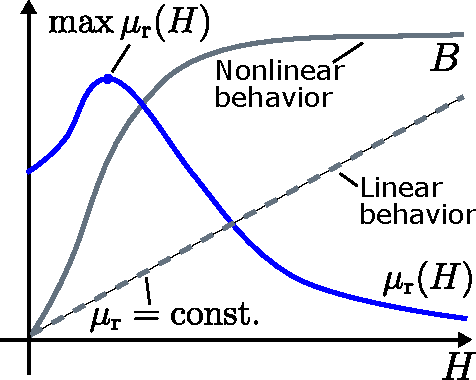
\includegraphics[height=0.5\textheight]{fig/lec02/Permeability_of_ferromagnet.pdf}
				\caption{Illustrative magnetisation curves for ferromagnets (and ferrimagnets) and corresponding permeabilities  (adapted from: \href{https://commons.wikimedia.org/wiki/File:Permeability_of_ferromagnet_by_Zureks.svg}{Wikimedia Commons}, public domain)}
			\end{figure}
		\end{column}
		\end{columns}
\end{frame}